Shape Analytics is a browser-based tool for exploring the stress, strain and deformation of elastic solids. It combines three levels of model: (i) a three-dimensional stress field built by superposing the Boussinesq and Cerruti half-space solutions over a load painted on the surface of a cuboid, cylinder or sphere; (ii) nine analytical simulators for classical problems (Mohr's circle, beams, shaft torsion, axial loading, pressure vessels, thermal stress, failure theories, energy methods and column buckling); and (iii) a finite element solver for bars, beams, plane-stress problems and a three-dimensional block.

This report states the theory behind each tool, shows how it is turned into code, and tests the code against independent results. The simulators reproduce closed-form solutions to the printed precision in every default case (Table~\ref{tab:defaults}). The finite element solver reproduces exact bar and beam solutions, converges at the expected rate (the four-node element is within $0.3\%$ of beam theory on eight elements through the depth), and recovers $K_t=3.06$ for a hole in a wide plate against the classical value of $3$.

\tableofcontents
\clearpage\pagenumbering{arabic}
\chapter{Introduction and system overview}
\label{ch:intro}

\section{Motivation and objectives}
Stress is not directly observable: it is a tensor with six independent components, and textbook solutions are closed forms for idealised geometries that hide the assumptions making them valid. The most instructive situations, such as a load on only part of a surface, have no simple closed form. This project builds an interactive tool that applies the governing equations to arbitrary inputs and states its assumptions. Its objectives are to
\begin{enumerate}[nosep]
\item compute and display the stress, strain and deformation inside a solid loaded over a user-painted patch of its surface (the \emph{3D stress field});
\item provide analytical simulators for nine canonical problems, each showing its governing equations beside the result;
\item provide a finite element solver against which the analytical results can be compared;
\item verify every component against closed-form results, limiting cases and invariants.
\end{enumerate}
All models are \textbf{linear elastic} with \textbf{small strain}, so superposition holds. The 3D field treats the body as an elastic half-space, which is exact for a body much larger than the loaded area; the finite element block (Section~\ref{sec:block}) measures the error otherwise. Plasticity, large rotation, contact and dynamics are out of scope.

\section{The software}
Shape Analytics is a browser application served by a small Python (FastAPI) server. It has three groups of tools, the \textbf{3D stress field} with section analytics, nine \textbf{analytical simulators}, and a \textbf{finite element tab}, all reached from one navigation bar (Figure~\ref{fig:ui-field}).

\begin{figure}[ht]
\centering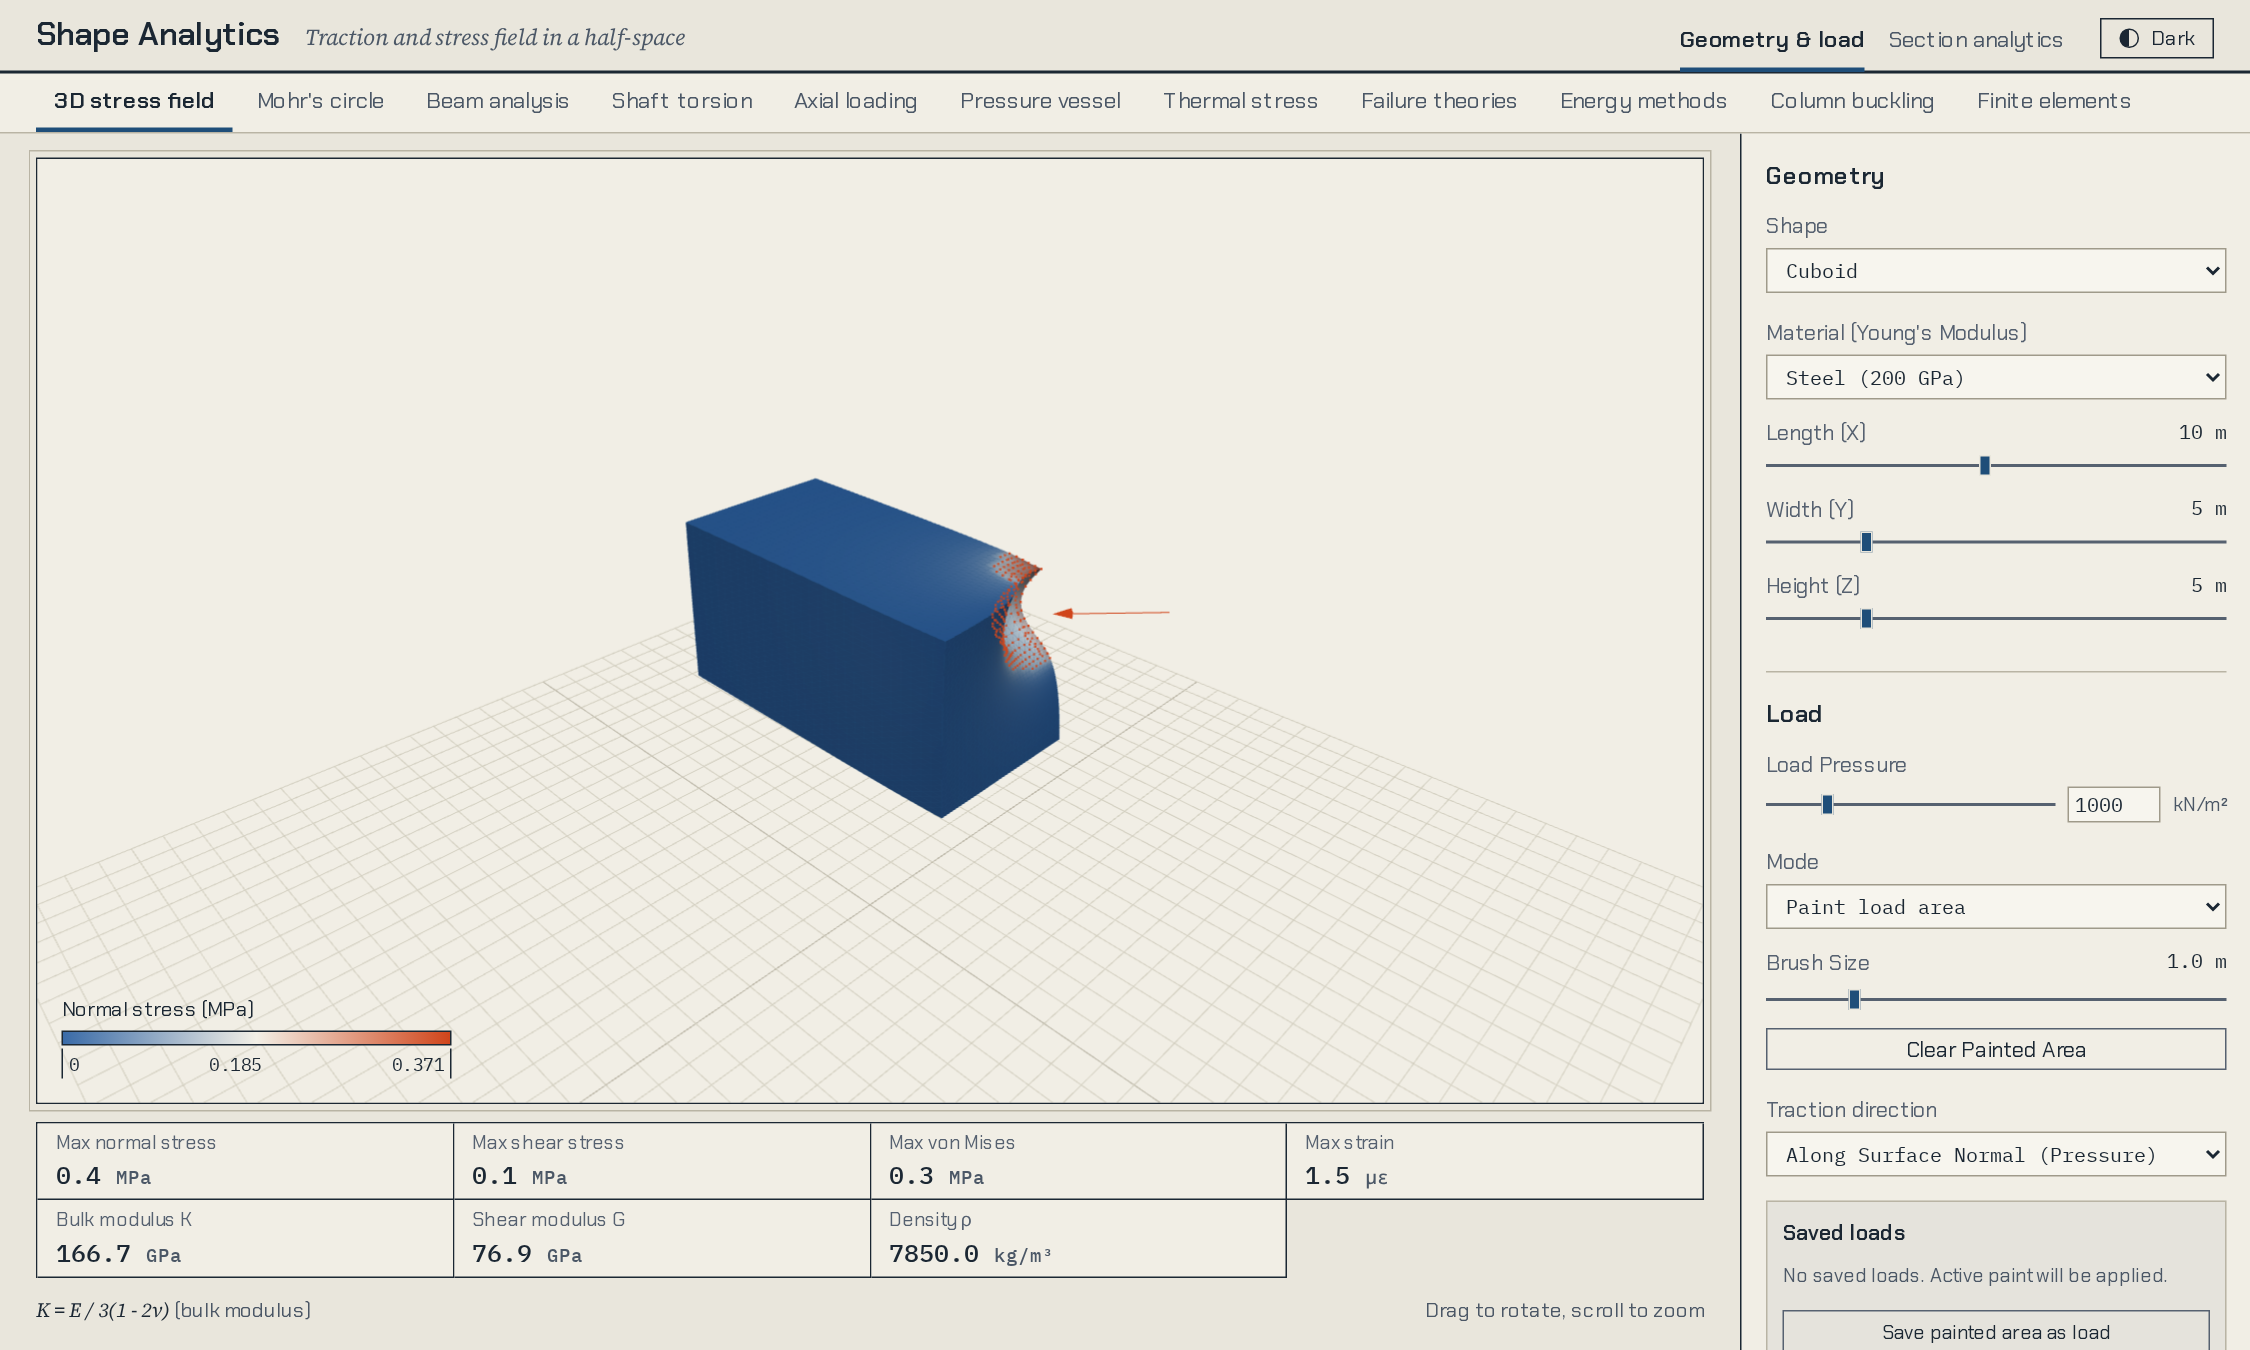
\includegraphics[width=0.9\linewidth]{../figures/ui_field_loaded.png}
\caption{The 3D stress field. A load painted on the top-right edge of a steel cuboid produces the coloured normal-stress map; the readout cards give the maxima of the displayed measures.}\label{fig:ui-field}
\end{figure}

\begin{center}\small
\begin{tabular}{@{}p{3.6cm}p{12cm}@{}}\toprule
File & Role\\\midrule
\file{index.html}, \file{style.css} & page structure, design tokens, light and dark themes\\
\file{app.js} & 3D field: geometry, painting, loads, stress computation, section plots\\
\file{physics.js} & half-space stresses and displacements, principal stresses, von Mises, strain\\
\file{sims.js} & the nine simulators as configuration objects, and the framework that renders them\\
\file{fem.js} & the FEM tab: controls, mesh drawing, charts, explanation panels\\
\file{server.py} & \texttt{/api/traction}, \texttt{/api/principal}, \texttt{/api/section}, static files\\
\file{fem.py}, \file{fem3d.py} & finite element solvers (bar, beam, 2D, 3D brick) and \texttt{/api/fem/solve}\\\bottomrule
\end{tabular}
\end{center}

\textbf{Conventions.} Tension is positive; in half-space frames $z$ points \emph{into} the body. The 3D field works in SI units internally and shows MPa; the simulators use mm, N and MPa; the FEM tab uses mm, kN and MPa in the interface and SI in the solver.

\begin{figure}[ht]
\centering
\resizebox{\linewidth}{!}{%
\begin{tikzpicture}[x=1cm,y=1cm,font=\footnotesize,
 box/.style={draw=accent,fill=white,rounded corners=1.5pt,align=center,inner sep=4pt,minimum width=2.7cm,minimum height=0.95cm},
 srv/.style={box,fill=paper},
 arr/.style={-{Stealth[length=2mm]},thick,draw=black!75},
 lab/.style={font=\scriptsize,fill=white,inner sep=1.5pt},
 grp/.style={draw=black!45,dashed,rounded corners=3pt,inner sep=7pt}]
\node[box] (html) at (0,0) {\file{index.html}\\layout, tabs};
\node[box] (lib)  at (0,-2.6) {Plotly, Three.js\\(CDN)};
\node[box] (app)  at (4.2,2.6) {\file{app.js}\\3D field};
\node[box] (sims) at (4.2,0) {\file{sims.js}\\9 simulators};
\node[box] (fem)  at (4.2,-2.6) {\file{fem.js}\\FEM tab};
\node[box] (phys) at (8.4,2.6) {\file{physics.js}\\half-space physics};
\node[srv] (srvr) at (12.9,0) {\file{server.py}\\FastAPI};
\node[srv] (femp) at (12.9,-2.6) {\file{fem.py}\\\file{fem3d.py}};
\begin{scope}[on background layer]
\node[grp,fit=(html)(lib)(app)(sims)(fem)(phys)] (browser) {};
\node[grp,fit=(srvr)(femp)] (server) {};
\end{scope}
\node[anchor=south west,font=\scriptsize\bfseries,text=black!60] at (browser.north west) {BROWSER};
\node[anchor=south west,font=\scriptsize\bfseries,text=black!60] at (server.north west) {SERVER};
\draw[thick,draw=black!75] (html.east) -- (2.15,0);
\draw[thick,draw=black!75] (2.15,2.6) -- (2.15,-2.6);
\draw[arr] (2.15,2.6) -- (app.west);
\draw[arr] (2.15,0) -- (sims.west);
\draw[arr] (2.15,-2.6) -- (fem.west);
\draw[arr] (html.south) -- node[lab,right=2pt]{loads} (lib.north);
\draw[arr] (fem.north) -- node[lab,right=2pt]{registerModule} (sims.south);
\draw[arr] (app.east) -- node[lab,above=1pt,fill=none]{imports} (phys.west);
\draw[arr] (app.north) -- ++(0,0.75) -| node[lab,pos=0.25]{POST /api/section} (srvr.north);
\draw[arr] (fem.east) -- node[lab,above=1pt,fill=none]{POST /api/fem/solve} (femp.west);
\draw[arr] (srvr.south) -- node[lab,right=2pt]{mounts router} (femp.north);
\end{tikzpicture}}
\caption{Architecture. The 3D field is computed in the browser (\file{physics.js}); only the section plots and the FEM solves call the server.}\label{fig:arch}
\end{figure}

There is no build step: the scripts are ES modules loaded by \file{index.html}, and \file{sims.js} and \file{fem.js} register themselves into the same navigation bar (Figure~\ref{fig:arch}). The 3D field runs entirely in the browser; the section plots and FEM solves go to the server because they evaluate thousands of points. The script \texttt{run\_shape\_analytics.sh} starts the server on port 8002, which also serves the page.
